\documentclass[11pt]{article}
\usepackage[utf8]{inputenc}
\usepackage[T1]{fontenc}
\usepackage{amsmath}
\usepackage{amssymb} % Needed for \eth
\usepackage{graphicx}
\usepackage{geometry}
\usepackage{tikz}
\usepackage{pgfplots} % For plots
\usepackage{ulem}     % For underline, using normalem to avoid messing with \emph
\usepackage{tcolorbox} % For boxing equations if needed
\usepackage{braket}    % For QM state notation if needed

\geometry{a4paper, margin=1in}
\usetikzlibrary{positioning, arrows.meta, shapes.geometric, patterns, calc} % Added calc library
\pgfplotsset{compat=1.18} % Use a recent PGFPlots version

% Custom commands (optional)
\newcommand{\avg}[1]{\overline{#1}}
\newcommand{\prob}[1]{P(#1)}
\newcommand{\ProbDens}[1]{\mathcal{P}(#1)} % Using script P for density
\newcommand{\vect}[1]{\vec{#1}}
\newcommand{\dd}[1]{\mathrm{d}#1} % Differential d
\newcommand{\pderiv}[2]{\frac{\partial #1}{\partial #2}}
\newcommand{\deriv}[2]{\frac{\mathrm{d} #1}{\mathrm{d} #2}}
\newcommand{\muState}{\mu\text{-state}} % Microstate
\newcommand{\OmegaE}{\Omega(E)}
\newcommand{\omegaE}{\omega(E)}
\newcommand{\PhiE}{\Phi(E)}
\newcommand{\deltaE}{\delta E}
\newcommand{\ethbar}{\text{\it{đ}}} % \eth symbol for inexact differential
\newcommand{\kb}{k_B} % Boltzmann constant
\newcommand{\gasR}{R} % Ideal gas constant
\newcommand{\partfn}{Z} % Partition function symbol
\newcommand{\grandpartfn}{\mathcal{Z}} % Grand partition function symbol
\newcommand{\lambdaT}{\lambda_{th}} % Thermal wavelength
\newcommand{\vrms}{v_{\text{RMS}}} % RMS speed
\newcommand{\vtilde}{\tilde{v}} % Most probable speed

\title{Physics 415 - Lecture 25: Maxwell Distribution and Kinetic Theory}
\date{March 19, 2025}
\author{} % Author not specified

\begin{document}

\maketitle
\thispagestyle{empty}

\section*{Summary}

\begin{itemize}
    \item Maxwell velocity distribution: $f(\vec{v}) = \left(\frac{m}{2\pi T}\right)^{3/2} e^{-m|\vec{v}|^2 / (2T)}$
    \item $f(\vec{v}) d^3v$ = probability that a gas particle has velocity in the range $(\vec{v}, \vec{v}+d^3v)$.
    \item (Derived in Lecture 18 by applying canonical distribution to a single gas molecule in equilibrium at temp $T$).
\end{itemize}
Summarize properties of $f(\vec{v})$ and use to deduce some simple properties of weakly interacting gases ("Kinetic Theory").

\section*{Properties of $f(\vec{v})$}

\begin{itemize}
    \item Factorization: $f(\vec{v})$ can be factorized:
    \[ f(\vec{v}) d^3v = [f_1(v_x) dv_x] [f_1(v_y) dv_y] [f_1(v_z) dv_z] \]
    where $f_1(v_i) = \sqrt{\frac{m}{2\pi T}} e^{-m v_i^2 / (2T)}$ for $i=x, y, z$.
    This means individual velocity components are statistically independent.

    \begin{center}
    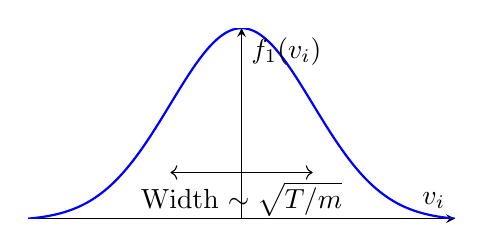
\begin{tikzpicture}
    \begin{axis}[
        xlabel=$v_i$, ylabel=$f_1(v_i)$,
        xtick={0}, ytick={0},
        axis lines=middle,
        width=7cm, height=4cm
    ]
    \addplot [domain=-3:3, samples=100, smooth, thick, blue] {sqrt(1/(2*pi))*exp(-x^2/2)}; % Scaled T/m=1
    \draw [<->] (axis cs:{-sqrt(1)}, 0.1) -- (axis cs:{sqrt(1)}, 0.1) node [midway, below] {Width $\sim \sqrt{T/m}$};
    \end{axis}
    \end{tikzpicture}
    \end{center}

    \item Averages involving $v_i$:
        \begin{itemize}
            \item $\avg{v_i} = \int_{-\infty}^{\infty} dv_i \, v_i f_1(v_i) = 0$ (integral of odd function).
            \item $\avg{v_i^2} = \int_{-\infty}^{\infty} dv_i \, v_i^2 f_1(v_i) = \sqrt{\frac{m}{2\pi T}} \int_{-\infty}^{\infty} v_i^2 e^{-m v_i^2 / (2T)} dv_i$.
            Using $\int_{-\infty}^{\infty} x^2 e^{-ax^2} dx = \frac{1}{2a}\sqrt{\frac{\pi}{a}}$ with $a=m/(2T)$:
            $\avg{v_i^2} = \sqrt{\frac{m}{2\pi T}} \left[ \frac{1}{2(m/2T)} \sqrt{\frac{\pi}{m/(2T)}} \right] = \sqrt{\frac{m}{2\pi T}} \left[ \frac{T}{m} \sqrt{\frac{2\pi T}{m}} \right] = \frac{T}{m}$.
            So, $\avg{v_i^2} = T/m$ for $i=x, y, z$.
        \end{itemize}
        This matches the equipartition theorem result: $\frac{1}{2} m \avg{v_i^2} = \frac{1}{2} T$. $\checkmark$

    \item Distribution for speed $v = |\vec{v}|$:
    Let $F(v) dv$ = probability that a gas particle has speed in the range $(v, v+dv)$.
    To find $F(v)$, integrate $f(\vec{v})$ over angles in spherical velocity coordinates ($d^3v = v^2 dv \sin\theta d\theta d\phi$).
    \[ F(v) dv = \left( \int_{\text{angles}} f(\vec{v}) v^2 \sin\theta d\theta d\phi \right) dv \]
    Since $f(\vec{v})$ only depends on $v^2$, it is isotropic. $\int \sin\theta d\theta d\phi = 4\pi$.
    \[ F(v) dv = f(v) \times 4\pi v^2 dv = 4\pi \left(\frac{m}{2\pi T}\right)^{3/2} v^2 e^{-m v^2 / (2T)} dv \]
    \[ F(v) = 4\pi \left(\frac{m}{2\pi T}\right)^{3/2} v^2 e^{-m v^2 / (2T)} \]

    \item Characteristic Speeds:
        \begin{itemize}
            \item Average speed $\avg{v}$: $\avg{v} = \int_0^\infty v F(v) dv$.
            $\avg{v} = 4\pi (\frac{m}{2\pi T})^{3/2} \int_0^\infty v^3 e^{-m v^2 / (2T)} dv$.
            Let $u^2 = mv^2/(2T)$, $v=\sqrt{2T/m} u$, $dv=\sqrt{2T/m} du$. Integral becomes $\int_0^\infty (\sqrt{2T/m}u)^3 e^{-u^2} (\sqrt{2T/m}du) = (\frac{2T}{m})^2 \int_0^\infty u^3 e^{-u^2} du$.
            Use $\int_0^\infty x^3 e^{-x^2} dx = 1/2$. Integral value is $(2T/m)^2 \times (1/2) = 2 T^2 / m^2$.
            $\avg{v} = 4\pi (\frac{m}{2\pi T})^{3/2} (\frac{2T^2}{m^2}) = 4\pi \frac{m^{3/2}}{(2\pi T)^{3/2}} \frac{2T^2}{m^2} = \frac{8\pi T^2 m^{3/2}}{ (2\pi T)^{3/2} m^2} = \sqrt{\frac{64 \pi^2 T^4 m^3}{8 \pi^3 T^3 m^4}} = \sqrt{\frac{8 T}{\pi m}}$.
            \[ \avg{v} = \sqrt{\frac{8T}{\pi m}} \approx 1.596 \sqrt{T/m} \]

            \item RMS speed $\vrms$: $\vrms = \sqrt{\avg{v^2}}$.
            $\avg{v^2} = \avg{v_x^2 + v_y^2 + v_z^2} = \avg{v_x^2} + \avg{v_y^2} + \avg{v_z^2} = T/m + T/m + T/m = 3T/m$.
            \[ \vrms = \sqrt{\frac{3T}{m}} \approx 1.732 \sqrt{T/m} \]
            (Matches equipartition $\frac{1}{2}m\avg{v^2} = \frac{3}{2}T$).

            \item Most probable speed $\vtilde$: Find $v$ where $F(v)$ is maximum. $\partial F / \partial v = 0$.
            Need $\partial/\partial v (v^2 e^{-m v^2 / (2T)}) = 0$.
            $(2v) e^{-m v^2 / (2T)} + v^2 e^{-m v^2 / (2T)} (-m v / T) = 0$.
            $2v - m v^3 / T = 0$. $2 = m v^2 / T$. $v^2 = 2T/m$.
            \[ \vtilde = \sqrt{\frac{2T}{m}} \approx 1.414 \sqrt{T/m} \]
        \end{itemize}
        Ordering: $\vtilde < \avg{v} < \vrms$.

    \begin{center}
    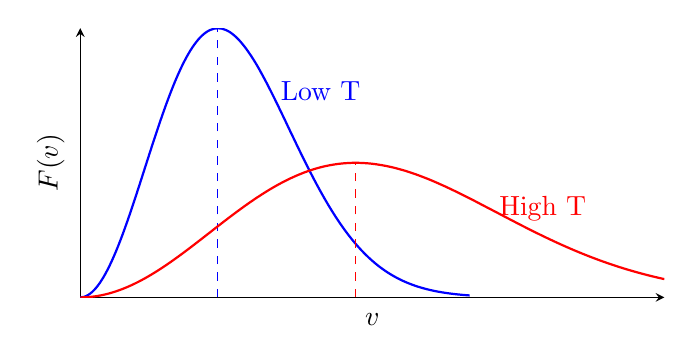
\begin{tikzpicture}
    \begin{axis}[
        xlabel={$v$}, ylabel=$F(v)$,
        xmin=0, ymin=0,
        xtick=\empty, ytick=\empty,
        axis lines=left, width=9cm, height=5cm,
        legend pos=north east
    ]
    % Scaled T=1
    \addplot [domain=0:4, samples=100, smooth, thick, blue] {4*pi*(1/(2*pi))^(1.5) * x^2 * exp(-x^2/2)} node[pos=0.5, anchor=west] {Low T};
    \draw [dashed, blue] (axis cs:{sqrt(2)}, 0) -- (axis cs:{sqrt(2)}, {4*pi*(1/(2*pi))^(1.5) * 2 * exp(-1)});
    % Scaled T=4
    \addplot [domain=0:6, samples=100, smooth, thick, red] {4*pi*(1/(8*pi))^(1.5) * x^2 * exp(-x^2/8)} node[pos=0.7, anchor=west] {High T};
    \draw [dashed, red] (axis cs:{sqrt(8)}, 0) -- (axis cs:{sqrt(8)}, {4*pi*(1/(8*pi))^(1.5) * 8 * exp(-1)});
    \node at (axis cs:1.414, -0.05) [blue] {$\tilde{v}$};
    \node at (axis cs:2.828, -0.05) [red] {$\tilde{v}$};
    \node at (axis cs:2.5, 0.7) {Higher T $\implies$ broader, peak shifts right};
    \end{axis}
    \end{tikzpicture}
    \end{center}
\end{itemize}

\section*{Simple Examples in Kinetic Theory}

"Kinetic Theory" = study of macroscopic properties of large numbers of particles starting from microscopic equations of motion (or distributions like $f(\vec{v})$). It can be used to study equilibrium and how systems reach equilibrium (transport phenomena). Here, only simplest equilibrium situations.

\subsection*{Number of Particles Striking a Surface (Flux)}

Calculate the number of particles striking a unit area of a wall per unit time.

Consider particles with velocity $\vec{v}$. In time $dt$, particles within a slanted cylinder based on area $dA$ on the wall, with height $v_z dt = (v \cos\theta) dt$ (where $\theta$ is angle to normal $\hat{z}$), will strike $dA$.
Volume of cylinder $= (v_z dt) dA$.
Number density of particles $n=N/V$.
Number of particles in this volume $= n (v_z dt dA)$.
Number of particles with velocity in $(\vec{v}, \vec{v}+d^3v)$ in this volume $= [f(\vec{v})d^3v] \times [n v_z dt dA]$.
(This is valid only for particles moving towards the wall, i.e., $v_z > 0$).

Let $\Phi(\vec{v}) d^3v$ be the number of particles with velocity $(\vec{v}, \vec{v}+d^3v)$ striking the wall \emph{per unit area per unit time}. Divide the above expression by $dA dt$:
\[ \Phi(\vec{v}) d^3v = n f(\vec{v}) v_z d^3v = n f(\vec{v}) (v \cos\theta) d^3v \quad (\text{for } v_z>0) \]
This is the differential particle flux.

The total particle flux $\Phi_0$ (particles per area per time) striking the wall is obtained by integrating $\Phi(\vec{v})$ over all velocities directed towards the wall ($v_z > 0$, or $\theta \in [0, \pi/2]$).
\[ \Phi_0 = \int_{v_z>0} \Phi(\vec{v}) d^3v = \int_{v_z>0} n f(\vec{v}) v_z d^3v \]
Use spherical coordinates $d^3v = v^2 dv \sin\theta d\theta d\phi$, $v_z = v \cos\theta$. $f(\vec{v})$ depends only on $v$.
\[ \Phi_0 = n \int_0^\infty dv \, v^2 f(v) \int_0^{\pi/2} d\theta \, \sin\theta \int_0^{2\pi} d\phi (v \cos\theta) \]
Angle integrals: $\int_0^{2\pi} d\phi = 2\pi$. $\int_0^{\pi/2} \sin\theta \cos\theta d\theta = [\frac{1}{2}\sin^2\theta]_0^{\pi/2} = 1/2$.
\[ \Phi_0 = n \int_0^\infty dv \, v^2 f(v) (v) (2\pi) (1/2) = \pi n \int_0^\infty v^3 f(v) dv \]
Recall the speed distribution $F(v) = 4\pi v^2 f(v)$ and average speed $\avg{v} = \int_0^\infty v F(v) dv = 4\pi \int_0^\infty v^3 f(v) dv$.
So, $\int_0^\infty v^3 f(v) dv = \avg{v} / (4\pi)$.
\[ \Phi_0 = \pi n (\avg{v} / (4\pi)) = \frac{1}{4} n \avg{v} \]
Using $\avg{v} = \sqrt{8T/(\pi m)}$:
\[ \Phi_0 = \frac{1}{4} n \sqrt{\frac{8T}{\pi m}} \]
Using ideal gas law $p = nT$ (with $T$ in energy units): $n=p/T$.
\[ \Phi_0 = \frac{p}{4T} \sqrt{\frac{8T}{\pi m}} = p \sqrt{\frac{8T}{16 \pi m T^2}} = p \sqrt{\frac{1}{2\pi m T}} \]
\[ \Phi_0 = \frac{p}{\sqrt{2\pi m T}} \]

\textbf{Application: Effusion}
Effusion is the process where molecules emerge from a small hole/slit in a container. "Small" means the hole does not significantly disturb the equilibrium of the gas inside.
If the hole has area $A$, the number of particles emerging per unit time (rate $I$) is:
\[ I = \Phi_0 \times A = \frac{p A}{\sqrt{2\pi m T}} \]
Since $I \propto 1/\sqrt{m}$, lighter molecules escape at a faster rate. This is used for isotopic separation (e.g., separating $^{235}$U from $^{238}$U for nuclear applications).

\subsection*{Pressure of Ideal Gas from Kinetic Theory}

Pressure arises from the momentum transfer of particles colliding with the walls.
Assume elastic collisions with a wall normal to $\hat{z}$. A particle with momentum $\vec{p}=m\vec{v}$ collides. $p_x, p_y$ are unchanged. $p_z \to -p_z$.
Change in particle momentum $\Delta \vec{p} = (0, 0, -2p_z)$.
Momentum imparted to the wall $= -\Delta \vec{p} = (0, 0, +2p_z)$. The momentum transferred is $2p_z = 2mv_z$ (in z-direction).

Consider particles with velocity $(\vec{v}, \vec{v}+d^3v)$ hitting area $dA$ in time $dt$.
Number hitting $= n f(\vec{v}) v_z d^3v \, dt \, dA$ (from flux calculation, for $v_z>0$).
Momentum transferred to wall by these particles in $dt$:
\[ dp_{\vec{v}, wall} = (\text{momentum per collision}) \times (\text{\# collisions}) \]
\[ dp_{\vec{v}, wall} = (2mv_z) \times (n f(\vec{v}) v_z d^3v \, dt \, dA) = 2mn v_z^2 f(\vec{v}) d^3v \, dt \, dA \]
Force on area $dA$ due to these particles: $dF_{\vec{v}} = dp_{\vec{v}, wall} / dt = 2mn v_z^2 f(\vec{v}) d^3v \, dA$.
Total force $F$ on area $dA$: Integrate over all velocities hitting the wall ($v_z>0$).
\[ F = \int_{v_z>0} dF_{\vec{v}} = \left( \int_{v_z>0} 2mn v_z^2 f(\vec{v}) d^3v \right) dA \]
Pressure $p = F/dA$:
\[ p = 2mn \int_{v_z>0} v_z^2 f(\vec{v}) d^3v \]
The integral $\int_{v_z>0} v_z^2 f(\vec{v}) d^3v$ is the average of $v_z^2$ for particles moving towards the wall ($v_z>0$). Since $f(\vec{v})$ depends only on $v^2$ (isotropic), the average for $v_z>0$ is the same as for $v_z<0$, and is half the average over all velocities:
\[ \int_{v_z>0} v_z^2 f(\vec{v}) d^3v = \frac{1}{2} \int v_z^2 f(\vec{v}) d^3v = \frac{1}{2} \avg{v_z^2} \]
\[ p = 2mn \left( \frac{1}{2} \avg{v_z^2} \right) = mn \avg{v_z^2} \]
Finally, using the equipartition result $\avg{v_z^2} = T/m$:
\[ p = mn (T/m) = nT \]
This recovers the ideal gas law $p=nT$ (or $pV=NT$) from kinetic theory. $\checkmark$

\end{document}